\providecommand{\main}{..}
\documentclass[../mthe-493-final-project.tex]{subfiles}

%Full analysis of results, against optimization constraints, and model measures like accuracy, staleness etc.

\begin{document}
    \chapter{Results \& Analysis}
    \label{ch:results-and-analysis}
    \section{Distributed Computing}
    %This may be best first, since it lets the reader now what accuracy the parameters fed into the optimization held.
    
    \section{Optimization}
    
    To test the efficacy of the heuristic optimization model, the solutions it produced in 10,000 experiments with varying parameters were compared against the solutions achieved by the Gurobi optimization tool. In 9.64\% of experiments both systems returned that there were no feasible points to the integer programming problem. Further, in all 10,000 experiments there were no disagreements between the models regarding problem feasibility. This indicates that the feasibility checks built into the heuristic model are completely exhaustive.
    
    
    \begin{figure}
        \centering
        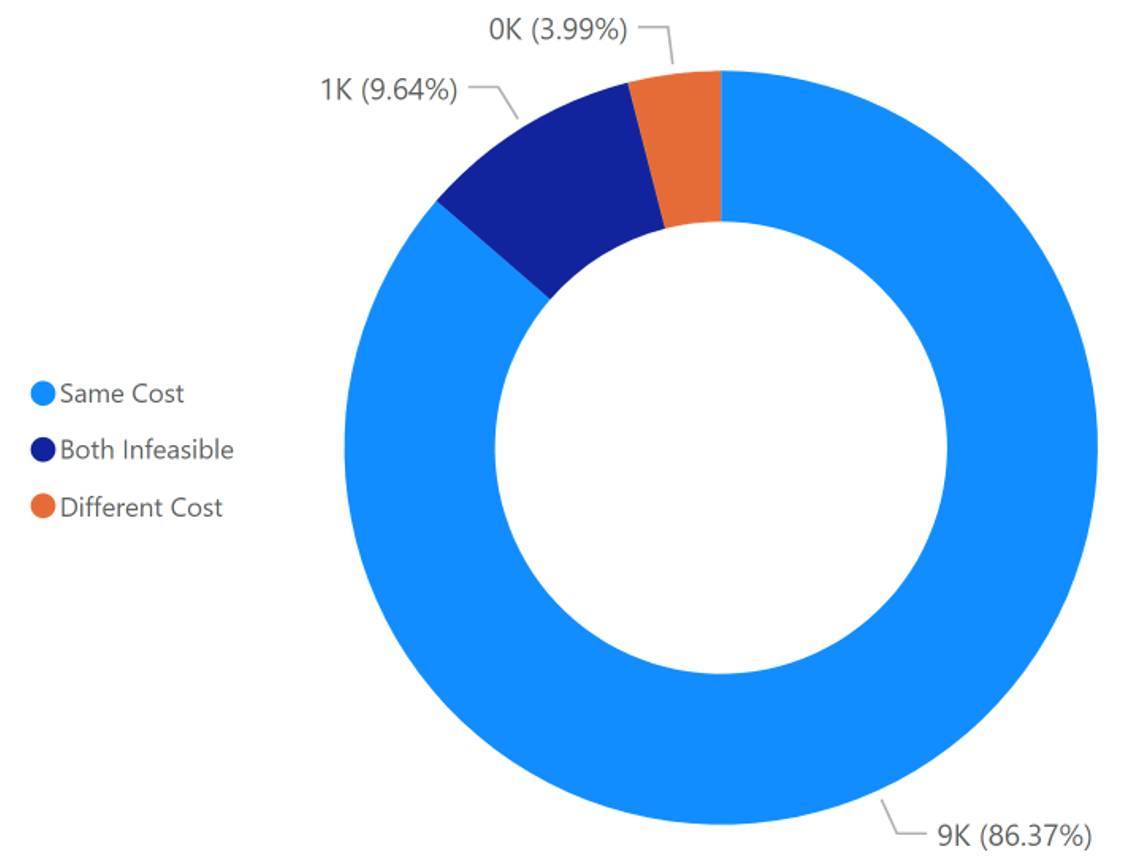
\includegraphics[width=120mm,scale=0.5]{optimization-results-1.png}
        \caption{Heuristic and Gurobi cost comparison over 10K experiments.}
        \label{fig:optimization-results-1}
    \end{figure}
    
    In 86.37\% of the 10,000 experiments both frameworks came to the same solution for minimal total deployment cost. This means that in 95.59\% of the cases where there was a feasible solution, both processes achieved the same optimum.
    
    In 4.42\% of the experiments for which there was a feasible solution, Gurobi and the heuristic model produced different results. Of these experiments, Gurobi achieved a lesser value in 49\%, while the heuristic model outperformed in the other 51\%.
    
    \begin{figure}
        \centering
        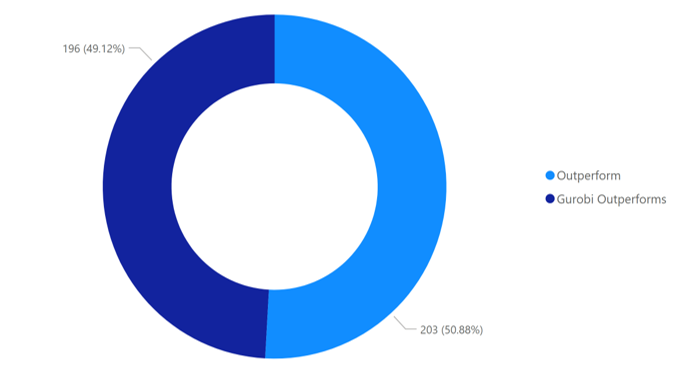
\includegraphics[width=150mm,scale=0.5]{optimization-results-2.png}
        \caption{Heuristic and Gurobi lower cost comparison in experiments with different results.}
        \label{fig:optimization-results-2}
    \end{figure}
    
    
    The fraction of cases where Gurobi outperforms is likely due to a small edge case which is not captured by the heuristic process. Conversely, in the cases where the heuristic model achieves a lower minimum for the objective function, it is speculated that this may be due to minute sacrifices in the accuracy of Gurobi's general-purpose optimizer in turn for speed increases. This cannot be confirmed because the Gurobi software is completely closed-source.
    
    Ultimately, the average difference between total costs in the experiments where the models produced different solutions was only 0.1\%. The largest recorded difference in total cost in a single experiment was 4\%.
    
    Since Gurobi is a widely trusted and reputable optimization engine~\cite{gurobi}, these results indicate that the heuristic model is also highly proficient as an optimizer.
    
    
    \section{Parallel Learning}

\end{document}
